% ============================================================
%  COM837 - ML for Wireless Communication, Assignment 3
%  Deep-Learning Channel Estimation (ChannelNet)
%  Satyaram Mangena (IMT2023576)
% ============================================================
\documentclass[a4paper,10pt]{article}

\usepackage[T1]{fontenc}
\usepackage{graphicx}
\usepackage{amsmath,amssymb,amsfonts}
\usepackage{geometry}
\usepackage{float}
\usepackage{booktabs}
\usepackage{subcaption}
\usepackage{enumitem}
\usepackage{xcolor}
\usepackage[colorlinks=true,linkcolor=blue,urlcolor=blue,citecolor=blue]{hyperref}

\geometry{a4paper, left=20mm, right=20mm, top=20mm, bottom=20mm}
\graphicspath{{figures/}{../figures/}{Images/}{../results/}}

\setlist{nosep,leftmargin=1.4em}

\title{\vspace{-1.6cm}\textbf{\Large Assignment 3 --- Deep-Learning Channel Estimation (ChannelNet)}\\[2pt]
\normalsize COM837: Machine Learning for Wireless Communication}
\author{\normalsize Satyaram Mangena (IMT2023576)}
\date{\vspace{-0.4cm}\small\today}

\begin{document}
\maketitle
\vspace{-0.7cm}

% ------------------------------------------------------------
\section{Overview}
% ------------------------------------------------------------
This assignment reproduces \textbf{ChannelNet} \cite{soltani2019}, which recasts
OFDM channel estimation as an image-reconstruction problem. The $72\times14$
time--frequency channel is treated as a two-channel (real/imaginary) image; the
noisy pilot observations, once interpolated to the full grid, are a blurred and
noisy ``low-resolution'' version of it. Two networks run in sequence: an
\emph{SRCNN} \cite{dong2016} sharpens the interpolated estimate, and a
\emph{DnCNN} \cite{zhang2017} removes the residual noise. I benchmark ChannelNet
against the classical LS\,+\,2-D interpolation estimator and against MMSE (both
an idealised and a practical variant), on the VehA and SUI5 channels, as a
function of SNR and pilot density.

Channels are generated in MATLAB with the Vienna 5G Link-Level Simulator
\cite{vienna}; estimation, training and evaluation are in Python/PyTorch. The
code is organised as a small library (\texttt{channelnet/}) with three entry
scripts: \texttt{run\_baselines.py} (Tasks~1--2), \texttt{run\_train.py}
(Tasks~3--5) and \texttt{run\_eval.py} (Task~6). Every experiment constant lives
in \texttt{channelnet/settings.py}, and each checkpoint stores its own
hyper-parameters, so the results can be regenerated from the saved weights
alone. The full source is available in my course repository~\cite{github}.

% ------------------------------------------------------------
\section{Dataset Generation (Task 1)}
% ------------------------------------------------------------
\paragraph{System model.} The SISO-OFDM subframe has $N_S=72$ subcarriers
($15$~kHz spacing, an LTE $1.4$~MHz allocation) and $N_D=14$ symbols. Each
resource element obeys
\begin{equation}
Y[i,k]=H[i,k]\,X[i,k]+Z[i,k],\qquad Z\sim\mathcal{CN}(0,\sigma^2).
\label{eq:model}
\end{equation}
Pilots are unit power and the channel is normalised to $\mathbb{E}|H|^2=1$, so
the operating SNR is simply $1/\sigma^2$.

\paragraph{Channels.} I use the simulator's \texttt{FastFading} class at a
$3.84$~MHz sampling rate ($256$-point FFT), sampling the transfer function at
the centre of each OFDM symbol and keeping the $72$ active subcarriers. The
carrier is $2.1$~GHz and the mobile speed $50$~km/h, giving a maximum Doppler of
about $97$~Hz (Jakes spectrum, $100$ sinusoids, independent subframes).
\textbf{VehA} is built in (RMS delay spread $\approx0.38~\mu$s). \textbf{SUI5}
is supplied as a user-defined power-delay profile: delays $0/4/10~\mu$s at
powers $0/{-}5/{-}10$~dB (RMS delay spread $\approx2.8~\mu$s). I generate
$40{,}000$ frames per model and split them $32{,}000/4{,}000/4{,}000$ into
train/val/test with one fixed permutation (seed~0). Each complex frame becomes
two real images (Fig.~\ref{fig:truth}).

\paragraph{Pilots.} I use diamond-lattice patterns (Fig.~\ref{fig:truth}c). The
main configuration has $48$ pilots, matching the LTE cell-specific reference
signal on antenna port~0 (pilot symbols $0,4,7,11$; every $6$th subcarrier; a
$3$-subcarrier stagger between pilot symbols). The density study adds the
$24$, $36$ and $72$ pilot layouts.

\begin{figure}[H]
\centering
\begin{subfigure}{0.32\textwidth}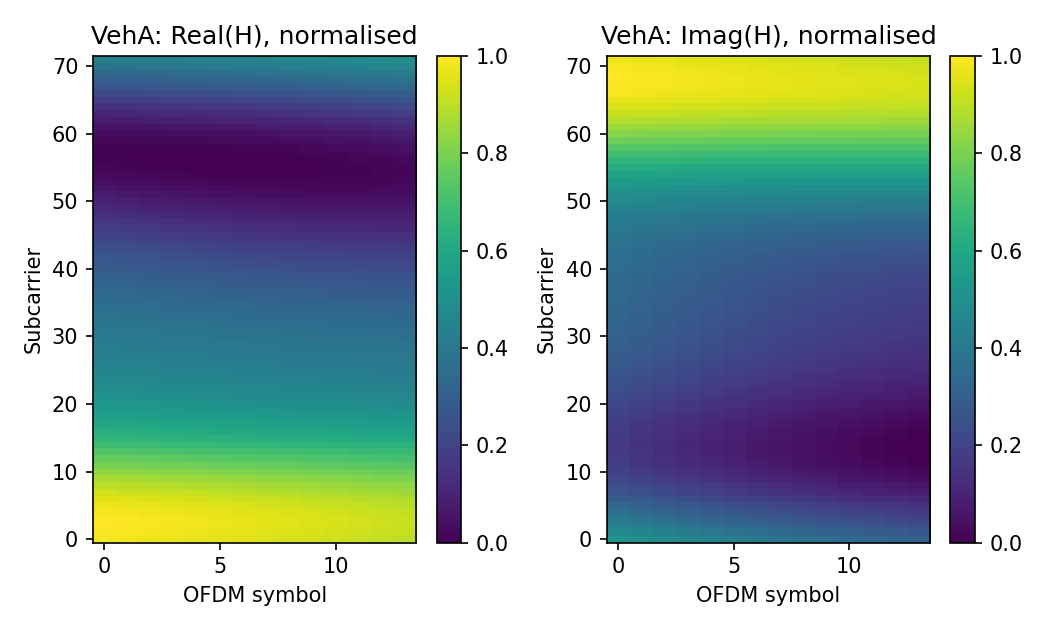
\includegraphics[width=\textwidth]{truth_VehA.png}\caption{VehA}\end{subfigure}\hfill
\begin{subfigure}{0.32\textwidth}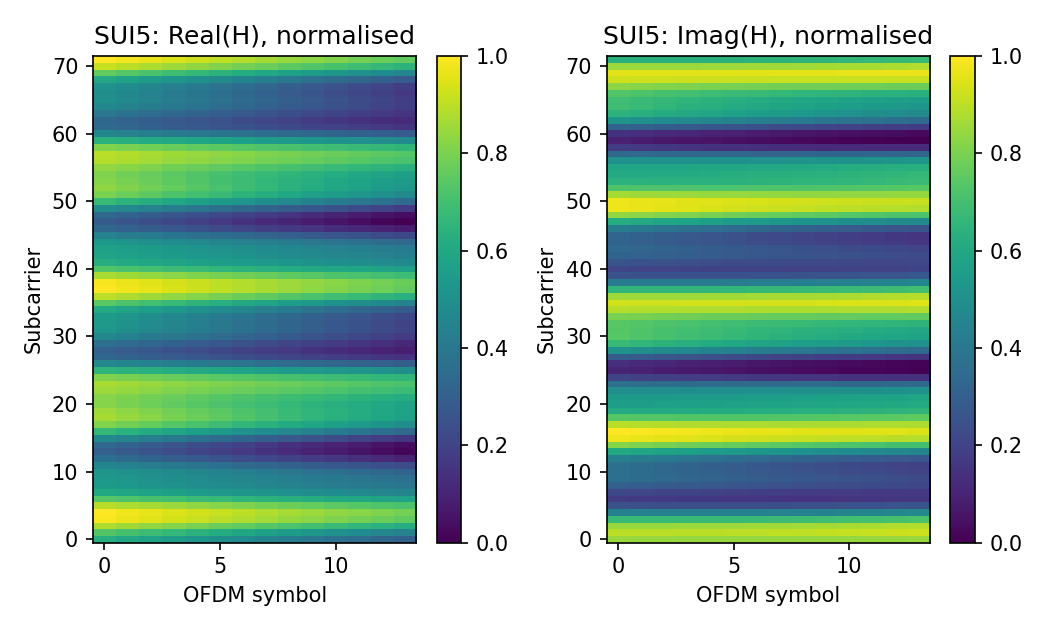
\includegraphics[width=\textwidth]{truth_SUI5.png}\caption{SUI5}\end{subfigure}\hfill
\begin{subfigure}{0.33\textwidth}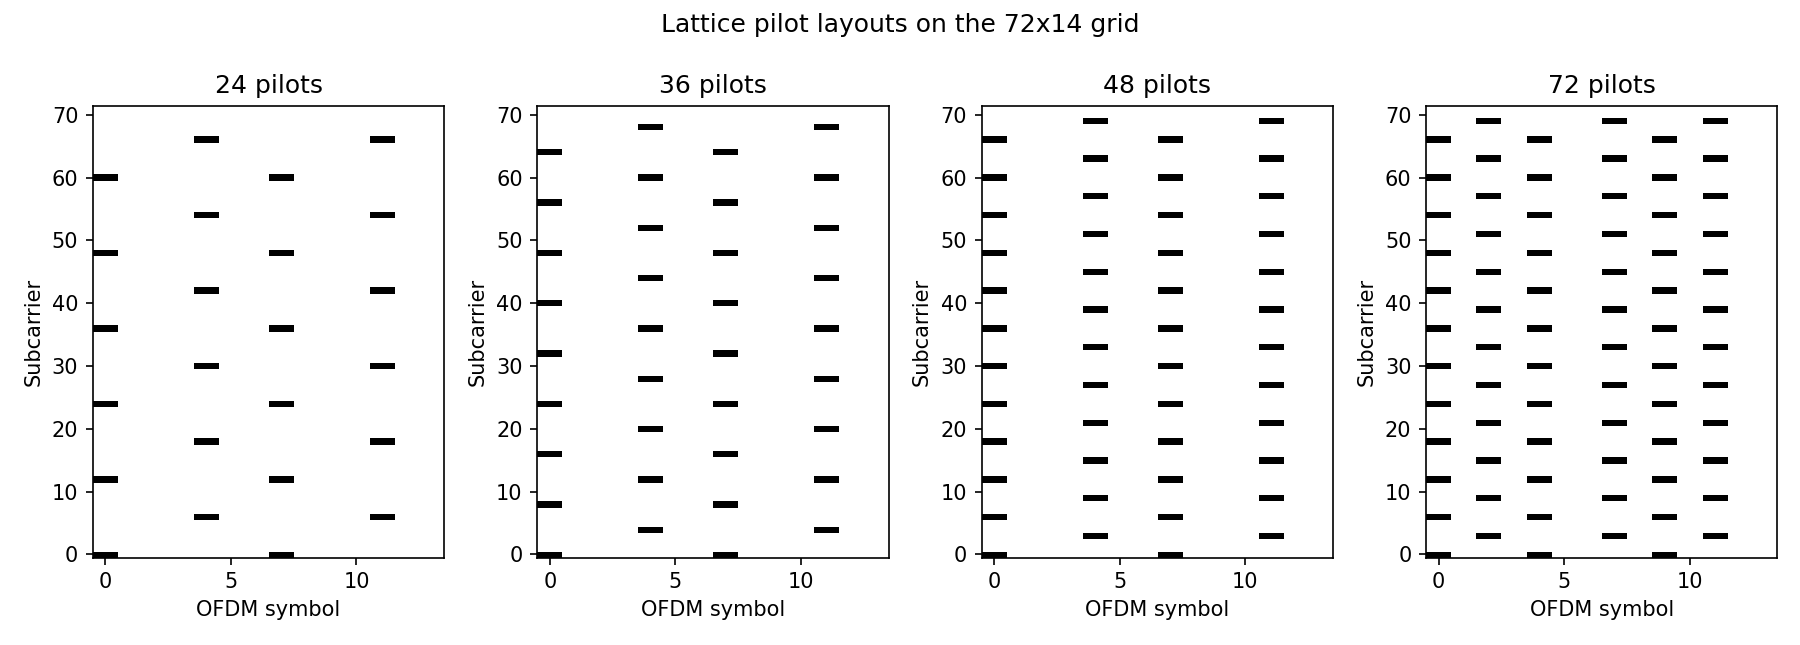
\includegraphics[width=\textwidth]{pilot_layouts.png}\caption{Pilot layouts}\end{subfigure}
\caption{Normalised real/imaginary channel images and the lattice pilot layouts.}
\label{fig:truth}
\end{figure}

\noindent VehA varies slowly across the grid. SUI5 shows pronounced frequency
stripes: its $10~\mu$s path makes the frequency response repeat roughly every
$100$~kHz ($\approx7$ subcarriers), which a pilot on every $6$th subcarrier can
barely resolve --- this is exactly what makes SUI5 the harder case below.

% ------------------------------------------------------------
\section{Classical Estimation (Task 2)}
% ------------------------------------------------------------
\paragraph{LS + interpolation.} At each pilot, $\hat h_{\mathrm{LS}}=Y/X=h+z$.
Because 2-D linear interpolation of scattered points is a linear map, I build it
once as a constant matrix $B\in\mathbb{R}^{1008\times N_p}$ (by interpolating the
unit vectors, with nearest-neighbour fill outside the pilots' convex hull) and
apply $\mathrm{vec}(\hat H)=B\,\hat h_{\mathrm{LS}}$ to every frame. This same
interpolated image is the input to SRCNN.

\paragraph{MMSE.} With unit pilots the linear MMSE estimator is
\begin{equation}
\hat h_{\mathrm{MMSE}}=A\,\hat h_{\mathrm{LS}},\qquad
A=R_{hp}\left(R_{pp}+\sigma^2 I\right)^{-1},
\end{equation}
with $R=\mathbb{E}[hh^{H}]$ the channel autocorrelation \cite{edfors1998}.
\emph{Ideal} MMSE takes $R$ from the $32{,}000$ true training channels --- a
lower reference no receiver can actually reach. \emph{Estimated} MMSE takes $R$
from only $1{,}000$ noisy interpolated frames, after subtracting the known noise
term $\sigma^2 BB^{T}$; this is the realistic counterpart. On SUI5, both LS and
estimated MMSE hit an error floor near $0.13$ (Table~\ref{tab:main}): linear
interpolation cannot track the fast frequency variation, and the estimated
statistics are learned from the same over-smoothed data.

% ------------------------------------------------------------
\section{ChannelNet and Training (Tasks 3--5)}
% ------------------------------------------------------------
\begin{table}[H]
\centering\small
\caption{ChannelNet architecture; `same' padding keeps the $72\times14$ size.}
\label{tab:arch}
\begin{tabular}{llr}
\toprule
\textbf{Stage} & \textbf{Layers} & \textbf{Params} \\
\midrule
SRCNN & Conv $9{\times}9$,64,ReLU $\to$ Conv $1{\times}1$,32,ReLU $\to$ Conv $5{\times}5$,1 & 8{,}129 \\
DnCNN & Conv $3{\times}3$,64,ReLU $\to$ $18{\times}$[Conv $3{\times}3$,64,BN,ReLU] $\to$ Conv $3{\times}3$,1 (residual) & 667{,}073 \\
\bottomrule
\end{tabular}
\end{table}

\paragraph{Two-stage training.} Stage~1 trains SRCNN to minimise
$C_1=\mathrm{mean}\,\|f_S(X)-H\|^2$, with $X$ the noisy interpolated LS image.
Stage~2 \emph{freezes} SRCNN, forms $Z=f_S(X)$, and trains DnCNN to minimise
$C_2=\mathrm{mean}\,\|f_R(Z)-H\|^2$. DnCNN learns residually: it predicts the
leftover noise $\hat n$ and outputs $Z-\hat n$. Real and imaginary parts are
fed through the same network as separate single-channel images, normalised by
the standard deviation of the target images so the loss is in unit-variance
units; the scale is undone before every reported MSE, so all MSEs are in
channel units.

Separate networks are trained per channel model and per SNR: $12$~dB
(``deep low-SNR'') and $22$~dB (``deep high-SNR''). The pilot study adds
networks for $24/36/72$ pilots at $12$~dB --- $20$ checkpoints in all. Training
uses Adam (lr $10^{-3}$, batch $128$), \texttt{ReduceLROnPlateau}, and early
stopping (patience $10$) with best-validation weights kept; SRCNN runs up to
$100$ epochs and DnCNN up to $40$ ($20$ for the pilot sweep). Train and
validation curves track each other closely in every run
(Fig.~\ref{fig:loss}), so there is no meaningful overfitting.

\begin{figure}[H]
\centering
\begin{subfigure}{0.49\textwidth}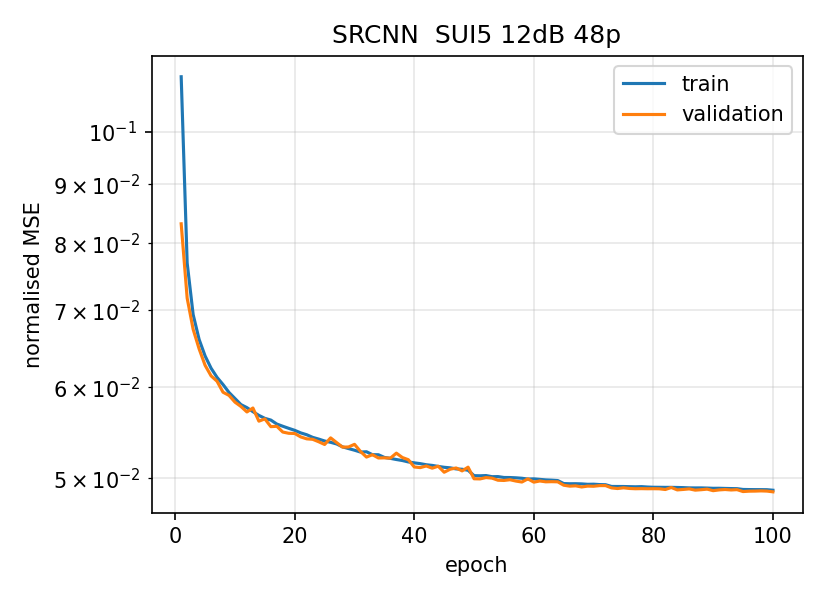
\includegraphics[width=\textwidth]{loss_SUI5_12dB_48p_sr.png}\caption{SRCNN stage, SUI5, 12 dB}\end{subfigure}\hfill
\begin{subfigure}{0.49\textwidth}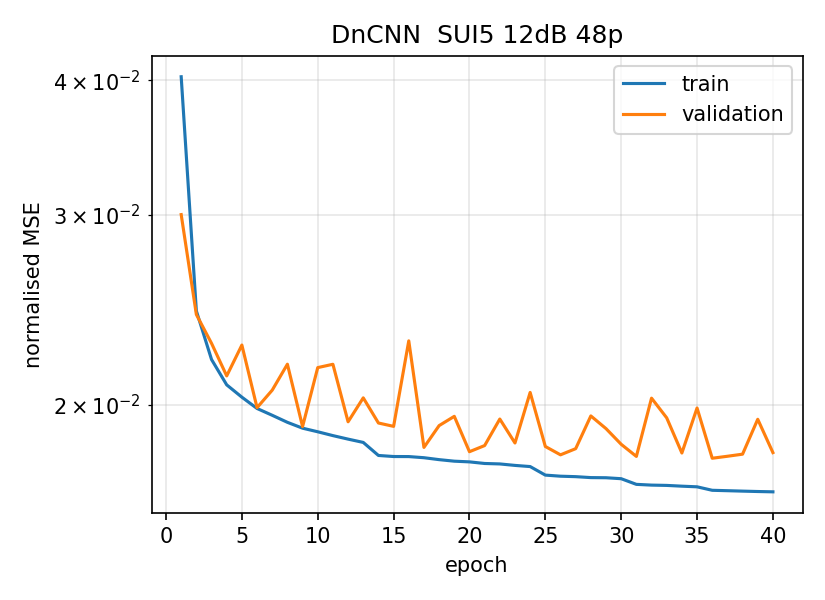
\includegraphics[width=\textwidth]{loss_SUI5_12dB_48p_dn.png}\caption{DnCNN stage, SUI5, 12 dB}\end{subfigure}
\caption{Representative training/validation loss curves (48 pilots).}
\label{fig:loss}
\end{figure}

\noindent The denoising stage matters most on SUI5: it is where the sharp
structure left by SRCNN is cleaned up, and the example images in
Fig.~\ref{fig:est} show the progression --- LS leaves blocky artefacts, SRCNN
recovers the structure but keeps noise, and DnCNN removes most of what remains.

% ------------------------------------------------------------
\section{Evaluation (Task 6)}
% ------------------------------------------------------------
\texttt{run\_eval.py} scores every method on the same $4{,}000$ test frames and
the same noise realisations, over $0$--$30$~dB in $2.5$~dB steps. Table~\ref{tab:main}
lists the headline $48$-pilot numbers and Fig.~\ref{fig:snr} plots the full
curves.\footnote{Values are from my run; \texttt{run\_eval.py} writes the full
sweep to \texttt{results/results.csv} and \texttt{results.json}.}

\begin{table}[H]
\centering\small
\caption{Test MSE (complex channel) vs SNR, 48 pilots.}
\label{tab:main}
\begin{tabular}{lccccccc}
\toprule
\textbf{Method} & \textbf{0 dB} & \textbf{5 dB} & \textbf{10 dB} & \textbf{15 dB} & \textbf{20 dB} & \textbf{25 dB} & \textbf{30 dB} \\
\midrule
\multicolumn{8}{l}{\textbf{VehA}}\\
LS + interp.        & 6.18e-1 & 1.97e-1 & 6.34e-2 & 2.12e-2 & 7.84e-3 & 3.61e-3 & 2.27e-3 \\
Estimated MMSE      & 1.04e-1 & 4.21e-2 & 1.72e-2 & 7.31e-3 & 3.68e-3 & 2.38e-3 & 1.91e-3 \\
Ideal MMSE          & 7.15e-2 & 3.19e-2 & 1.28e-2 & 4.89e-3 & 1.84e-3 & 6.72e-4 & 2.43e-4 \\
ChannelNet (12 dB)  & 1.66e-1 & 5.22e-2 & 1.78e-2 & 7.46e-3 & 4.23e-3 & 3.21e-3 & 2.88e-3 \\
ChannelNet (22 dB)  & 7.62e-1 & 1.15e-1 & 2.73e-2 & 8.24e-3 & 2.79e-3 & 1.11e-3 & 5.79e-4 \\
\midrule
\multicolumn{8}{l}{\textbf{SUI5}}\\
LS + interp.        & 7.46e-1 & 3.24e-1 & 1.91e-1 & 1.48e-1 & 1.35e-1 & 1.31e-1 & 1.30e-1 \\
Estimated MMSE      & 2.01e-1 & 1.54e-1 & 1.37e-1 & 1.31e-1 & 1.30e-1 & 1.29e-1 & 1.29e-1 \\
Ideal MMSE          & 6.71e-2 & 2.69e-2 & 1.02e-2 & 3.67e-3 & 1.28e-3 & 4.30e-4 & 1.50e-4 \\
ChannelNet (12 dB)  & 2.58e-1 & 7.66e-2 & 2.60e-2 & 1.08e-2 & 5.97e-3 & 4.45e-3 & 3.95e-3 \\
ChannelNet (22 dB)  & 4.41e-1 & 1.25e-1 & 3.66e-2 & 1.15e-2 & 4.00e-3 & 1.69e-3 & 9.72e-4 \\
\bottomrule
\end{tabular}
\end{table}

\begin{figure}[H]
\centering
\begin{subfigure}{0.49\textwidth}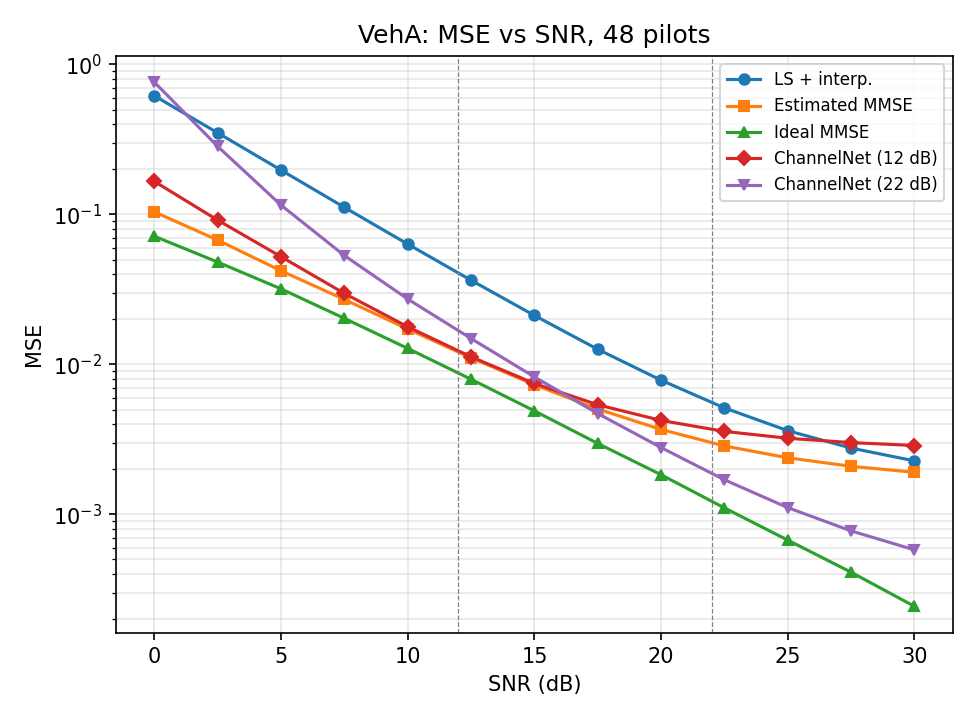
\includegraphics[width=\textwidth]{mse_snr_VehA.png}\caption{VehA}\end{subfigure}\hfill
\begin{subfigure}{0.49\textwidth}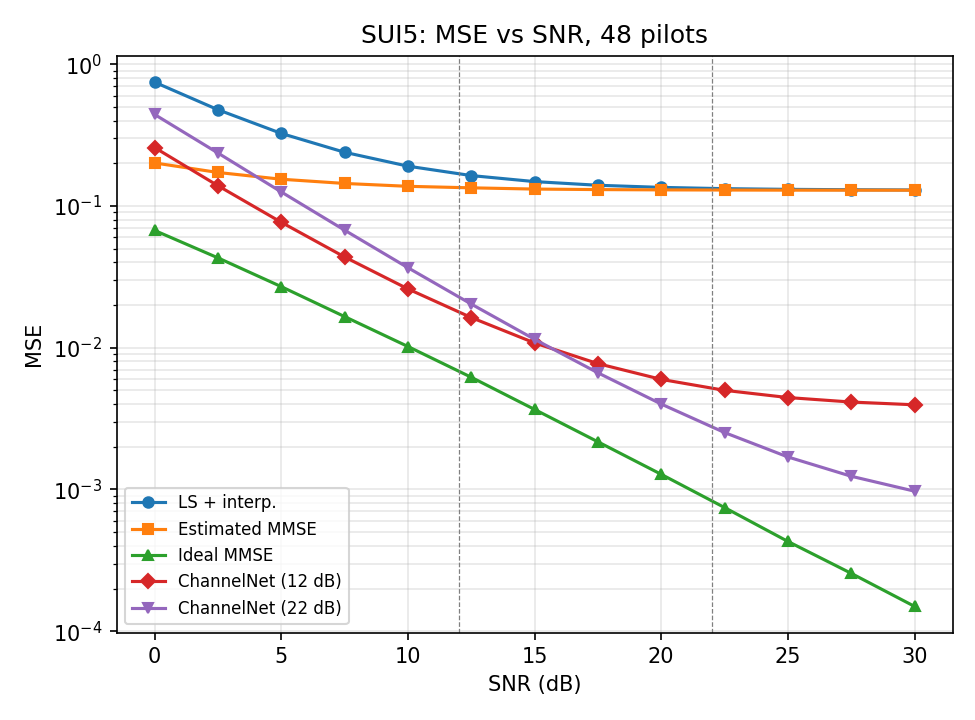
\includegraphics[width=\textwidth]{mse_snr_SUI5.png}\caption{SUI5}\end{subfigure}
\caption{MSE vs SNR, 48 pilots; dashed lines mark the two training SNRs.}
\label{fig:snr}
\end{figure}

\paragraph{VehA.} ChannelNet beats LS at every SNR. The $12$~dB network roughly
matches estimated MMSE below $15$~dB; the $22$~dB network overtakes it above
$\approx17$~dB, reaching $5.8\mathrm{e}{-4}$ at $30$~dB against $1.9\mathrm{e}{-3}$
for estimated MMSE ($\approx3.3\times$). Ideal MMSE stays the lower bound,
matching the paper's conclusion that ChannelNet is \emph{comparable} to
practical MMSE on VehA.

\paragraph{SUI5.} This is the clear win. ChannelNet removes the $\approx0.13$
interpolation floor entirely: at $25$~dB it reaches $1.7\mathrm{e}{-3}$, roughly
\textbf{two orders of magnitude} below LS and estimated MMSE. This reproduces
the paper's headline result that ChannelNet substantially outperforms
approximated MMSE on a highly frequency-selective channel.

\begin{figure}[H]
\centering
\begin{subfigure}{0.49\textwidth}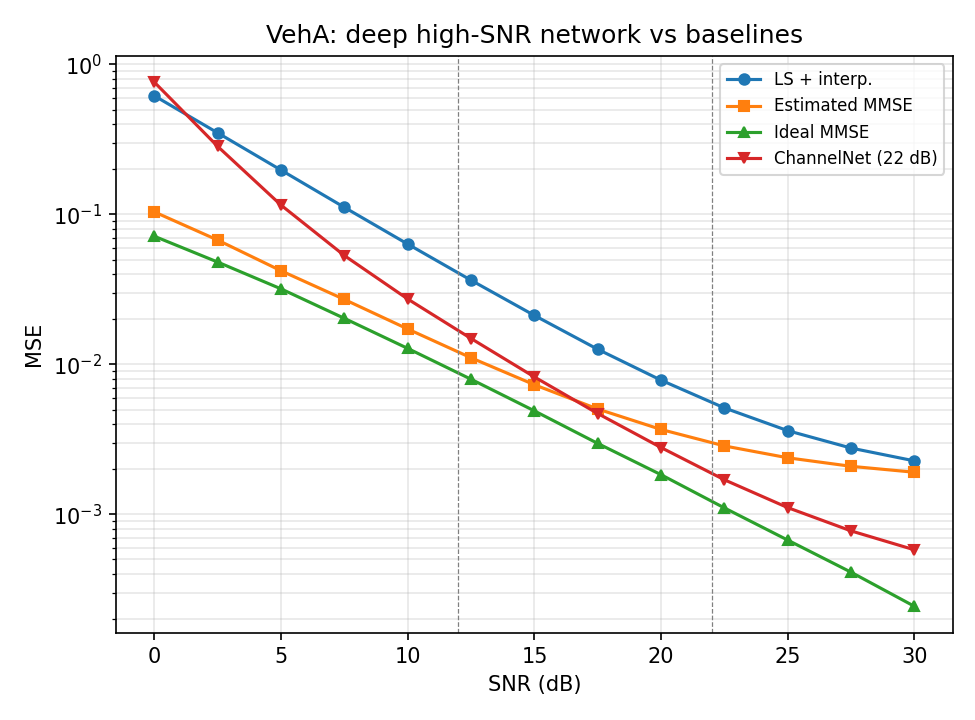
\includegraphics[width=\textwidth]{highsnr_VehA.png}\caption{VehA}\end{subfigure}\hfill
\begin{subfigure}{0.49\textwidth}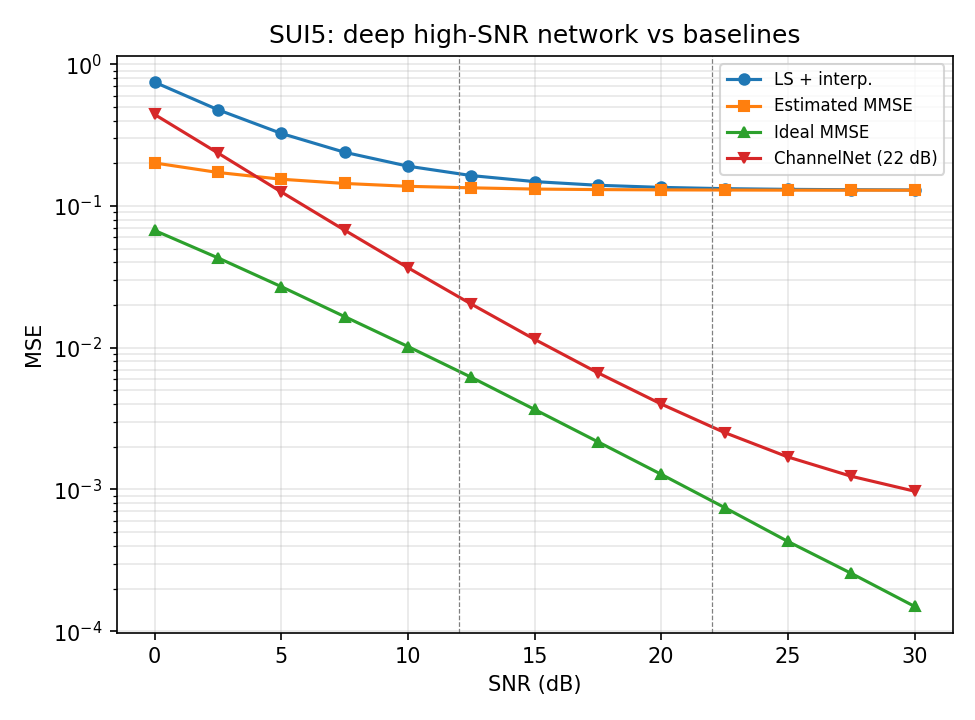
\includegraphics[width=\textwidth]{highsnr_SUI5.png}\caption{SUI5}\end{subfigure}
\caption{Deep high-SNR network (22 dB) against the classical baselines.}
\label{fig:highsnr}
\end{figure}

\begin{figure}[H]
\centering
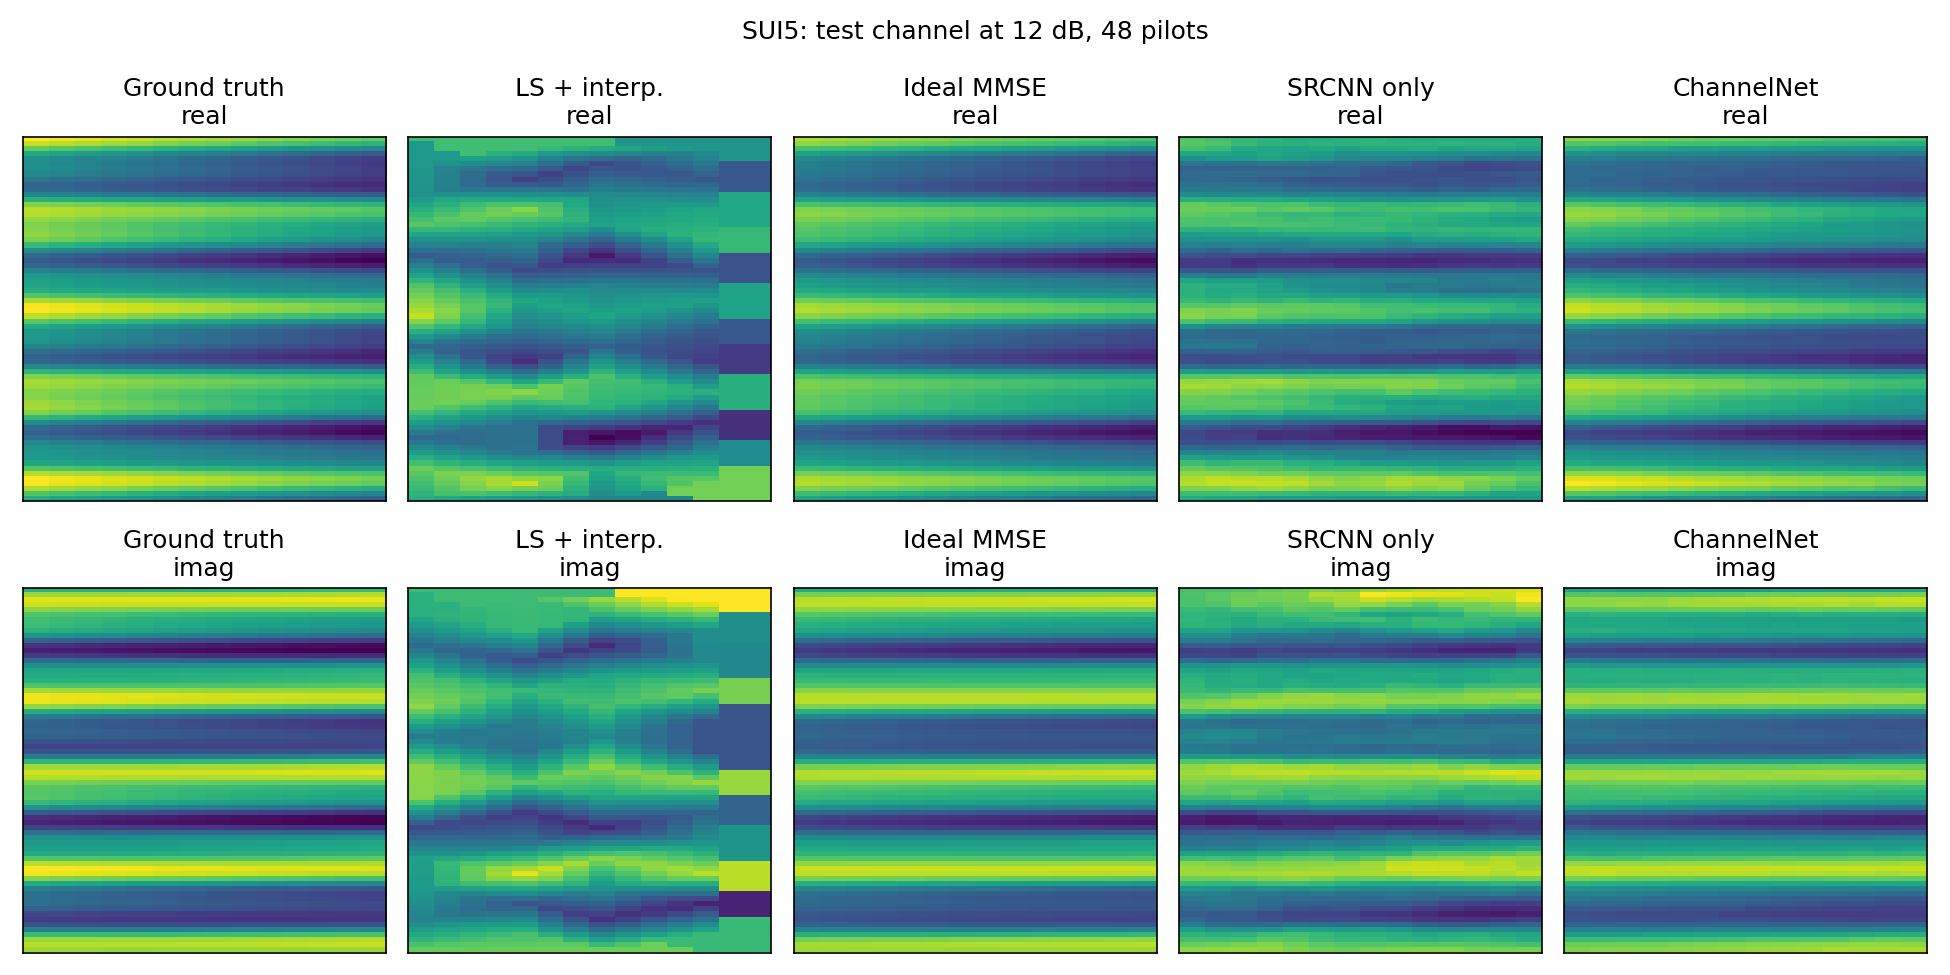
\includegraphics[width=0.9\textwidth]{estimates_SUI5.png}
\caption{SUI5 at 12 dB: truth, LS+interp., ideal MMSE, SRCNN only, full ChannelNet.}
\label{fig:est}
\end{figure}

\begin{figure}[H]
\centering
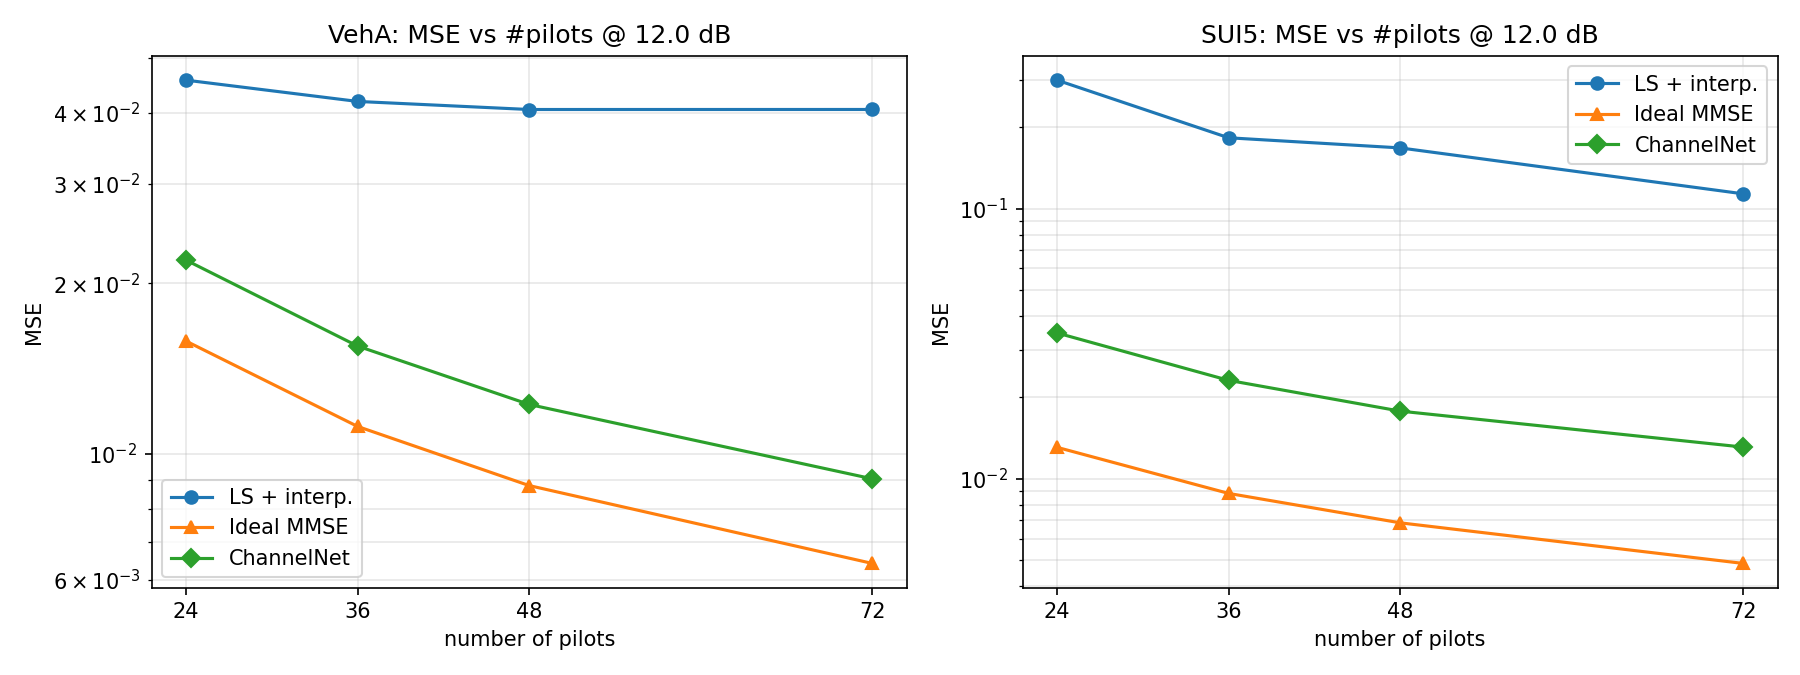
\includegraphics[width=0.78\textwidth]{mse_pilots.png}
\caption{MSE vs number of pilots at 12 dB (one ChannelNet per pilot count).}
\label{fig:pilots}
\end{figure}

\paragraph{Pilot density.} ChannelNet improves steadily with more pilots
(Fig.~\ref{fig:pilots}). On VehA, LS is nearly flat because at $12$~dB it is
noise-limited rather than spacing-limited; on SUI5 LS improves strongly with
density as the stripes become resolvable. Crucially, ChannelNet on SUI5 with
only $24$ pilots already beats LS with $72$ pilots, so the learned estimator can
trade pilot overhead for computation. (The sweep networks used at most $20$
DnCNN epochs, so their points are mildly pessimistic.)

% ------------------------------------------------------------
\section{Discussion}
% ------------------------------------------------------------
\paragraph{Q1 --- Limitations of SNR-specific training and their effect on
generalisation.} Each network is dependable only near its training SNR:
\begin{itemize}
\item \textbf{High-SNR network at low SNR.} The $22$~dB model never saw strong
noise, so its denoiser passes most of it through. At $0$~dB on VehA it is
\emph{worse than plain LS} ($0.76$ vs $0.62$), and on SUI5 it trails the $12$~dB
model up to about $15$~dB.
\item \textbf{Low-SNR network at high SNR.} The $12$~dB model learned to smooth
aggressively; when noise is small this erases genuine detail and creates a
floor. On VehA at $30$~dB it again falls behind LS, and on SUI5 it saturates
near $4\mathrm{e}{-3}$ while the $22$~dB model reaches $9.7\mathrm{e}{-4}$.
\item \textbf{Deployment cost.} The two curves cross around $15$--$17$~dB, so a
receiver needs an SNR estimate and a bank of stored networks (or must accept a
mismatch penalty). A simple switch at $17$~dB (my ``switched'' curve) always
picks the better of the two, but two training points cover $0$--$30$~dB only
coarsely. Networks are also tied to one pilot pattern and one channel model,
multiplying how many must be stored.
\end{itemize}

\paragraph{Q2 --- Improving generalisation across SNR.}
\begin{itemize}
\item \textbf{Multi-SNR (blind) training:} train one network on frames whose SNR
is drawn across the whole range; the blind DnCNN-B \cite{zhang2017} nearly
matches noise-specific models.
\item \textbf{Noise-conditioned networks:} supply $\sigma^2$ (or an estimated
SNR) as an extra input map, as FFDNet does \cite{zhang2018ffdnet}, so one
network adapts its smoothing --- an OFDM receiver can estimate SNR cheaply.
\item \textbf{Network bank with switching/blending:} store a few SNR-specific
models and select or interpolate by estimated SNR (simple, memory-hungry).
\item \textbf{Model-driven designs:} unrolled estimators with learned denoisers
or LS-refining residual networks generalise across SNR better than black-box
mappings.
\item \textbf{Online adaptation / joint pilot design:} meta-learning for fast
few-shot adaptation, and learning pilot placement jointly with the estimator to
reduce how much super-resolution is needed.
\end{itemize}

% ------------------------------------------------------------
\section{Limitations and Conclusion}
% ------------------------------------------------------------
\textbf{Limitations.} SUI5 is approximated with a Jakes Doppler rather than the
standard rounded SUI spectrum; the frequency-domain model
(Eq.~\ref{eq:model}) ignores ICI/ISI even though SUI5's $10~\mu$s path exceeds
the $\approx4.7~\mu$s cyclic prefix; ideal MMSE is an unrealisable reference; and
DnCNN ($667$k parameters) is far more costly at inference than LS or a
precomputed MMSE matrix, with one network needed per SNR, pilot pattern and
channel model.

\textbf{Conclusion.} I reproduced ChannelNet end to end. On VehA it matches
practical MMSE at low SNR and beats it at high SNR; on the frequency-selective
SUI5 channel it removes the LS/estimated-MMSE error floor, with up to two orders
of magnitude lower MSE. Its principal weakness is SNR specificity, for which
multi-SNR or noise-conditioned training is the most direct remedy.

% ------------------------------------------------------------
{\small
\begin{thebibliography}{9}
\bibitem{soltani2019} M.~Soltani, V.~Pourahmadi, A.~Mirzaei, H.~Sheikhzadeh,
``Deep Learning-Based Channel Estimation,'' \textit{IEEE Commun.\ Lett.}, vol.~23,
no.~4, pp.~652--655, 2019.
\bibitem{dong2016} C.~Dong, C.~C.~Loy, K.~He, X.~Tang, ``Image Super-Resolution
Using Deep Convolutional Networks,'' \textit{IEEE TPAMI}, vol.~38, no.~2,
pp.~295--307, 2016.
\bibitem{zhang2017} K.~Zhang, W.~Zuo, Y.~Chen, D.~Meng, L.~Zhang, ``Beyond a
Gaussian Denoiser: Residual Learning of Deep CNN for Image Denoising,''
\textit{IEEE TIP}, vol.~26, no.~7, pp.~3142--3155, 2017.
\bibitem{vienna} S.~Pratschner \textit{et al.}, ``Versatile Mobile
Communications Simulation: The Vienna 5G Link Level Simulator,'' \textit{EURASIP
J.\ Wireless Commun.\ Netw.}, 2018:226, 2018.
\bibitem{edfors1998} O.~Edfors \textit{et al.}, ``OFDM Channel Estimation by
Singular Value Decomposition,'' \textit{IEEE Trans.\ Commun.}, vol.~46, no.~7,
pp.~931--939, 1998.
\bibitem{zhang2018ffdnet} K.~Zhang, W.~Zuo, L.~Zhang, ``FFDNet: Toward a Fast
and Flexible Solution for CNN-Based Image Denoising,'' \textit{IEEE TIP},
vol.~27, no.~9, pp.~4608--4622, 2018.
\bibitem{github} S.~Mangena, ``MLWC\_assignment\_3,'' GitHub repository.
[Online]. Available: \url{https://github.com/Satya968/MLWC_assignment_3}
\end{thebibliography}
}
\end{document}
